\documentclass{article}%
\usepackage[T1]{fontenc}%
\usepackage[utf8]{inputenc}%
\usepackage{lmodern}%
\usepackage{textcomp}%
\usepackage{lastpage}%
\usepackage{parskip}%
\usepackage[top=1.2in,bottom=1in,left=0.6in,right=0.6in,headsep=0.8in]{geometry}%
\usepackage{amsmath}%
\usepackage{graphicx}%
\usepackage{needspace}%
\usepackage{color}%
\usepackage{longtable}%
\usepackage{multirow}%
\usepackage[table]{xcolor}%
\usepackage{fancyhdr}%
\usepackage{tabularx}%
%
\definecolor{OsdagGreen}{HTML}{D5DF93}%
\fancypagestyle{header}{ 
\renewcommand{\headrulewidth}{0pt}%
\renewcommand{\footrulewidth}{0pt}%
\fancyhead{ 
}%
\fancyfoot{ 
}%
\fancyhead[C]{ 
\begin{tabularx}{\textwidth}{|l|p{6cm}|l|X|}%
\hline%
\rowcolor{OsdagGreen}%
Company Name&&Project Title&\\%
\hline%
\rowcolor{OsdagGreen}%
Group/Team Name&&Subtitle&\\%
\hline%
\rowcolor{OsdagGreen}%
Designer&&Job Number&\\%
\hline%
\rowcolor{OsdagGreen}%
Date&04 /05 /2020&Client&\\%
\hline%
\end{tabularx}
}%
\fancyfoot[R]{ 
Page \thepage\ of \pageref{LastPage}
}
}%
%
\begin{document}%
\normalsize%
\pagestyle{header}%
\section{Input Parameters}%
\label{sec:InputParameters}%
\renewcommand{\arraystretch}{1.2}%
\begin{longtable}{|p{5cm}|p{2cm}|p{2cm}|p{2cm}|p{5cm}|}%
\hline%
\hline%
\multicolumn{3}{|c|}{Module}&\multicolumn{2}{|c|}{Beam Coverplate  Weld Connection}\\%
\hline%
\hline%
\multicolumn{3}{|c|}{MainModule}&\multicolumn{2}{|c|}{Moment Connection}\\%
\hline%
\hline%
\multicolumn{3}{|c|}{Moment(kNm)*}&\multicolumn{2}{|c|}{9.0}\\%
\hline%
\hline%
\multicolumn{3}{|c|}{Shear(kN)*}&\multicolumn{2}{|c|}{9.0}\\%
\hline%
\hline%
\multicolumn{3}{|c|}{Axial (kN) *}&\multicolumn{2}{|c|}{9.0}\\%
\hline%
\hline%
\multicolumn{5}{|c|}{\textbf{Section}}\\%
\hline%
\hline%
\multirow{13}{*}{\includegraphics[width=5cm,height=5cm]{"C:/Users/Priti/Desktop/Osdag3/ResourceFiles/images/ISection".png}}&\multicolumn{2}{|c|}{Beam Section *}&\multicolumn{2}{|c|}{UB 305 x 165 x 46}\\%
\cline{2%
-%
5}%
&\multicolumn{2}{|c|}{Material *}&\multicolumn{2}{|c|}{E 250 (Fe 410 W)A}\\%
\cline{2%
-%
5}%
&\multicolumn{2}{|c|}{Ultimate strength, fu (MPa)}&\multicolumn{2}{|c|}{410}\\%
\cline{2%
-%
5}%
&\multicolumn{2}{|c|}{Yield Strength , fy (MPa)}&\multicolumn{2}{|c|}{230}\\%
\cline{2%
-%
5}%
&Mass&46.1&Iz(mm4)&98990000.0\\%
\cline{2%
-%
5}%
&Area(mm2) {-} A&5870.0&Iy(mm4)&8960000.0\\%
\cline{2%
-%
5}%
&D(mm)&307.0&rz(mm)&130.0\\%
\cline{2%
-%
5}%
&B(mm)&165.7&ry(mm)&39.0\\%
\cline{2%
-%
5}%
&t(mm)&6.7&Zz(mm3)&646000.0\\%
\cline{2%
-%
5}%
&T(mm)&11.8&Zy(mm3)&108000.0\\%
\cline{2%
-%
5}%
&FlangeSlope&90&Zpz(mm3)&720000.0\\%
\cline{2%
-%
5}%
&R1(mm)&8.9&Zpy(mm3)&108000.0\\%
\cline{2%
-%
5}%
&R2(mm)&0.0&&\\%
\cline{2%
-%
5}%
\hline%
\multicolumn{5}{|c|}{\textbf{Weld Details}}\\%
\hline%
\hline%
\multicolumn{3}{|c|}{Weld Type}&\multicolumn{2}{|c|}{Fillet}\\%
\hline%
\hline%
\multicolumn{3}{|c|}{Type of weld fabrication}&\multicolumn{2}{|c|}{Shop Weld}\\%
\hline%
\hline%
\multicolumn{3}{|c|}{Material grade overwrite (MPa) Fu}&\multicolumn{2}{|c|}{410.0}\\%
\hline%
\end{longtable}

%
\Needspace{10\baselineskip}%
\section{Design Checks}%
\label{sec:DesignChecks}%
\subsection{Member Capacity}%
\label{subsec:MemberCapacity}%
\renewcommand{\arraystretch}{1.2}%
\begin{longtable}{|p{4cm}|p{5cm}|p{5.5cm}|p{1.5cm}|}%
\hline%
\rowcolor{OsdagGreen}%
Check&Required&Provided&Remarks\\%
\hline%
\endhead%
\hline%
Axial Capacity Member Ac (kN)&&$\begin{aligned} Ac &=\frac{A*f_y}{\gamma_{m0} *1000}\\ &=\frac{5870.0*230}{1.1* 1000}\\ &=1227.36\end{aligned}$&\\%
\hline%
\end{longtable}

%
\subsection{Member Capacity}%
\label{subsec:MemberCapacity}%
\renewcommand{\arraystretch}{1.2}%
\begin{longtable}{|p{4cm}|p{5cm}|p{5.5cm}|p{1.5cm}|}%
\hline%
\rowcolor{OsdagGreen}%
Check&Required&Provided&Remarks\\%
\hline%
\endhead%
\hline%
Axial Capacity Member Ac (kN)&&$\begin{aligned} Ac &=\frac{A*f_y}{\gamma_{m0} *1000}\\ &=\frac{5870.0*230}{1.1* 1000}\\ &=1227.36\end{aligned}$&\\%
\hline%
Shear Capacity Member Sc (kN)&&$\begin{aligned} S_c &= \frac{A_v*f_y}{\sqrt{3}*\gamma_{mo} *1000}\\ &=\frac{283.4*6.7*230}{\sqrt{3}*1.1 *1000}\\ &=229.21823999999998\end{aligned}$&\\%
\hline%
Plastic Moment Capacity Pmc (kNm)&&$\begin{aligned} Pmc &= \frac{\beta_b * Z_p *fy}{\gamma_{mo} * 1000000}\\ &=\frac{1*134529*230}{1.1 * 1000000}\\ &=28.13\end{aligned}$&\\%
\hline%
Moment Deformation Criteria Mdc (kNm)&&$\begin{aligned} Mdc &= \frac{1.5 *Z_e *fy}{1.1}\\ &= \frac{1.5 *646000.0*230}{1.1}\\ &= 202.61\end{aligned}$&\\%
\hline%
Moment Capacity Member Mc (kNm)&&$\begin{aligned} M_c &= min(Pmc,Mdc)\\ &=min(28.13,202.61)\\ &=28.13\end{aligned}$&\\%
\hline%
\end{longtable}

%
\subsection{Load Considered}%
\label{subsec:LoadConsidered}%
\renewcommand{\arraystretch}{1.2}%
\begin{longtable}{|p{4cm}|p{5cm}|p{5.5cm}|p{1.5cm}|}%
\hline%
\rowcolor{OsdagGreen}%
Check&Required&Provided&Remarks\\%
\hline%
\endhead%
\hline%
Applied Axial Load Au (kN)&$\begin{aligned} Ac_{min} &= 0.3 * A_c\\ &= 0.3 *1227.36\\ &=368.21\end{aligned}$&$\begin{aligned} Au &= max(A,Ac_{min} )\\ &= max( 9.0,368.21)\\ &=368.21\end{aligned}$&Pass\\%
\hline%
Applied Shear Load Vu (kN)&$\begin{aligned} Sc_{min} &= 0.6 * A_c\\ &= 0.6 *229.22\\ &=137.53\end{aligned}$&$\begin{aligned} Vu &= max(V,Vc_{min})\\ &=  max(9.0,137.53)\\ &=137.53\end{aligned}$&Pass\\%
\hline%
Applied Moment Load Mu (kNm)&$\begin{aligned} Mc_{min} &= 0.5 * M_c\\ &= 0.5 *28.13\\ &=14.06\end{aligned}$&$\begin{aligned} Mu &= max(M,Mc_{min} )\\ &= max(9.0,14.06)\\ &=14.06\end{aligned}$&Pass\\%
\hline%
Forces Carried by Web&&$\begin{aligned}A_w &= Axial~ force~ in~ web  \\   &= \frac{(D- 2*T)*t* Au }{A} \\ &= \frac{(307.0- 2*11.8)*6.7*368.21 }{5870.0} \\ &=119.11\\ M_w &= Moment ~in ~web  \\  &= \frac{Z_w * Mu}{Z} \\ &= \frac{134529 * 14.06}{720000.0} \\ &=2.63\end{aligned}$&\\%
\hline%
Forces Carried by Flange&&$\begin{aligned} A_f&= Axial~force~ in ~flange  \\ &= \frac{Au * B *T}{A} \\ &= \frac{368.21 * 165.7*11.8}{5870.0} \\ &=122.65\\ M_f& =Moment~ in~ flange \\  & = Mu-M_w\\ &= 14.06-2.63\\ &=11.44\\  f_f& =flange~force  \\ & = \frac{M_f *1000}{D-T} + A_f \\ &= \frac{11.44}{307.0-11.8} +122.65 \\ &=161.39\end{aligned}$&\\%
\hline%
Shear Capacity Member Sc (kN)&&$\begin{aligned} S_c &= \frac{A_v*f_y}{\sqrt{3}*\gamma_{mo} *1000}\\ &=\frac{283.4*6.7*230}{\sqrt{3}*1.1 *1000}\\ &=229.21823999999998\end{aligned}$&\\%
\hline%
Plastic Moment Capacity Pmc (kNm)&&$\begin{aligned} Pmc &= \frac{\beta_b * Z_p *fy}{\gamma_{mo} * 1000000}\\ &=\frac{1*134529*230}{1.1 * 1000000}\\ &=28.13\end{aligned}$&\\%
\hline%
Moment Deformation Criteria Mdc (kNm)&&$\begin{aligned} Mdc &= \frac{1.5 *Z_e *fy}{1.1}\\ &= \frac{1.5 *646000.0*230}{1.1}\\ &= 202.61\end{aligned}$&\\%
\hline%
Moment Capacity Member Mc (kNm)&&$\begin{aligned} M_c &= min(Pmc,Mdc)\\ &=min(28.13,202.61)\\ &=28.13\end{aligned}$&\\%
\hline%
\end{longtable}

%
\subsection{Load Considered}%
\label{subsec:LoadConsidered}%
\renewcommand{\arraystretch}{1.2}%
\begin{longtable}{|p{4cm}|p{5cm}|p{5.5cm}|p{1.5cm}|}%
\hline%
\rowcolor{OsdagGreen}%
Check&Required&Provided&Remarks\\%
\hline%
\endhead%
\hline%
Applied Axial Load Au (kN)&$\begin{aligned} Ac_{min} &= 0.3 * A_c\\ &= 0.3 *1227.36\\ &=368.21\end{aligned}$&$\begin{aligned} Au &= max(A,Ac_{min} )\\ &= max( 9.0,368.21)\\ &=368.21\end{aligned}$&Pass\\%
\hline%
Applied Shear Load Vu (kN)&$\begin{aligned} Sc_{min} &= 0.6 * A_c\\ &= 0.6 *229.22\\ &=137.53\end{aligned}$&$\begin{aligned} Vu &= max(V,Vc_{min})\\ &=  max(9.0,137.53)\\ &=137.53\end{aligned}$&Pass\\%
\hline%
Applied Moment Load Mu (kNm)&$\begin{aligned} Mc_{min} &= 0.5 * M_c\\ &= 0.5 *28.13\\ &=14.06\end{aligned}$&$\begin{aligned} Mu &= max(M,Mc_{min} )\\ &= max(9.0,14.06)\\ &=14.06\end{aligned}$&Pass\\%
\hline%
Forces Carried by Web&&$\begin{aligned}A_w &= Axial~ force~ in~ web  \\   &= \frac{(D- 2*T)*t* Au }{A} \\ &= \frac{(307.0- 2*11.8)*6.7*368.21 }{5870.0} \\ &=119.11\\ M_w &= Moment ~in ~web  \\  &= \frac{Z_w * Mu}{Z} \\ &= \frac{134529 * 14.06}{720000.0} \\ &=2.63\end{aligned}$&\\%
\hline%
Forces Carried by Flange&&$\begin{aligned} A_f&= Axial~force~ in ~flange  \\ &= \frac{Au * B *T}{A} \\ &= \frac{368.21 * 165.7*11.8}{5870.0} \\ &=122.65\\ M_f& =Moment~ in~ flange \\  & = Mu-M_w\\ &= 14.06-2.63\\ &=11.44\\  f_f& =flange~force  \\ & = \frac{M_f *1000}{D-T} + A_f \\ &= \frac{11.44}{307.0-11.8} +122.65 \\ &=161.39\end{aligned}$&\\%
\hline%
\end{longtable}

%
\subsection{Flange Weld  Design Check }%
\label{subsec:FlangeWeldDesignCheck}%
\renewcommand{\arraystretch}{1.2}%
\begin{longtable}{|p{4cm}|p{6cm}|p{5.5cm}|p{1.5cm}|}%
\hline%
\rowcolor{OsdagGreen}%
Check&Required&Provided&Remarks\\%
\hline%
\endhead%
\hline%
Min Weld Size (mm)&$\begin{aligned} &Thickness~of~Thicker~part\\ \noindent &=max(11.8,11.8)\\ &=18.0\\ &IS800:2007~cl.10.5.2.3~Table 21,\\  &t_{w_{min}}=5\end{aligned}$&10&Pass\\%
\hline%
Max Weld Size (mm)&$\begin{aligned} Thickness~of~Thinner~part&\\ =Min(11.8,11.8)&=11.8\\ t_{w_{max}} &=11.8\end{aligned}$&10&Pass\\%
\hline%
\end{longtable}

%
\subsection{ Outer Flange  plate Check }%
\label{subsec:OuterFlangeplateCheck}%
\renewcommand{\arraystretch}{1.2}%
\begin{longtable}{|p{4cm}|p{6cm}|p{5.5cm}|p{1.5cm}|}%
\hline%
\rowcolor{OsdagGreen}%
Check&Required&Provided&Remarks\\%
\hline%
\endhead%
\hline%
Min. Plate Height (mm)&$\begin{aligned} b_{fp} &= \{B - 2*sp} \\ &= \{165.7 - 2 * 15} \ &=135\end{aligned}$&115&Fail\\%
\hline%
Min. Plate Length (mm)&$\begin{aligned} l_{fp} & = [ 2*(l_wl + 2*s) + g]\\ &= + \frac{10.0}]\\ &=420\end{aligned}$&185&Fail\\%
\hline%
\end{longtable}

%
\subsection{Inner and Outer flange plate Checks}%
\label{subsec:InnerandOuterflangeplateChecks}%
\renewcommand{\arraystretch}{1.2}%
\begin{longtable}{|p{4cm}|p{6cm}|p{5.5cm}|p{1.5cm}|}%
\hline%
\rowcolor{OsdagGreen}%
Check&Required&Provided&Remarks\\%
\hline%
\endhead%
\hline%
Min. Plate Height (mm)&$\begin{aligned} b_{fp} &= \{B - 2*sp} \\ &= \{165.7 - 2 * 15} \ &=135\end{aligned}$&115&Fail\\%
\hline%
Min. Plate Length (mm)&$\begin{aligned} l_{fp} & = [ 2*(l_wl + 2*s) + g]\\ &= + \frac{10.0}]\\ &=420\end{aligned}$&185&Fail\\%
\hline%
\end{longtable}

%
\subsection{Web Weld  Design Check }%
\label{subsec:WebWeldDesignCheck}%
\renewcommand{\arraystretch}{1.2}%
\begin{longtable}{|p{4cm}|p{6cm}|p{5.5cm}|p{1.5cm}|}%
\hline%
\rowcolor{OsdagGreen}%
Check&Required&Provided&Remarks\\%
\hline%
\endhead%
\hline%
Min Weld Size (mm)&$\begin{aligned} &Thickness~of~Thicker~part\\ \noindent &=max(6.7,6.7)\\ &=6.7\\ &IS800:2007~cl.10.5.2.3~Table 21,\\  &t_{w_{min}}=3\end{aligned}$&10&Pass\\%
\hline%
Max Weld Size (mm)&$\begin{aligned} Thickness~of~Thinner~part&\\ =Min(6.7,6.7)&=6.0\\ t_{w_{max}} &=6.0\end{aligned}$&10&Fail\\%
\hline%
\end{longtable}

%
\Needspace{10\baselineskip}%
\newpage%
\section{3D View}%
\label{sec:3DView}%


\begin{figure}[h!]%
\centering%
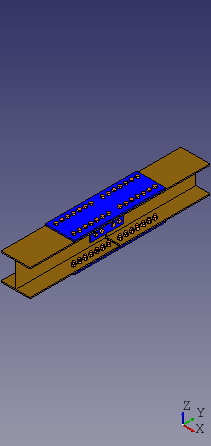
\includegraphics[width=\linewidth]{{"C:/Users/Priti/Desktop/Osdag3./ResourceFiles/images/3d}.png}%
\caption{3D View}%
\end{figure}

%
\end{document}